\documentclass[preprint,11pt]{elsarticle}

\usepackage{lmodern}
\usepackage{amsmath,amssymb,amsthm}
\usepackage{booktabs}
\usepackage{graphicx}
\usepackage[hidelinks]{hyperref}
\input{glyphtounicode}
\pdfgentounicode=1

\newtheorem{theorem}{Theorem}
\newtheorem{proposition}{Proposition}
\newcommand{\E}{\mathbb E}
\newcommand{\Prb}{\mathbb P}
\newcommand{\given}{\mathcal F}
\newcommand{\pos}[1]{\left[#1\right]_+}

\begin{document}
\begin{frontmatter}

\title{Finite-sample certificates for the Bayes accuracy gain of feature fusion in QUIC traffic}
\author{Anonymous authors}
\date{}

\begin{abstract}
We derive finite-sample lower bounds on the gain in class-weighted Bayes accuracy when an additional feature augments a discrete representation. The guarantee is conditional on a fixed evaluation cohort and a rule fitted in a separate period. It assumes conditional independence across blocks and permits arbitrary dependence within blocks. Nested features yield nonnegative cell gains, which we bound simultaneously and sum. For 44 classes in CESNET-QUICEXT-25 XS, the pooled product bounds on the gain from adding packet timing are 2.035 and 1.935 percentage points under daily blocks in two disjoint evaluation windows. After omitting the cell with the largest original contribution and correcting for selection among omissions, the daily bounds are 0.405 and 0.298 points. Across calendar alignments in the second window, four-day bounds range from zero to 1.229 points. For 16 classes, the daily cell product bounds are 1.483 and 2.327 points, with nearly all of the bound from one cell in each window. The two primary daily bounds in the second window have at least 95\% joint conditional coverage. On CESNET-QUIC22-S, daily bounds reach 1.289 points, and two- and four-day bounds are zero. Controlled simulations show how gain concentration and the number of occupied cells affect the relative performance of the cell and pooled bounds.
\end{abstract}

\begin{keyword}
Information fusion \sep Bayes accuracy \sep finite-sample inference \sep block dependence \sep encrypted traffic
\end{keyword}
\end{frontmatter}

\section{Introduction}

Classifiers for encrypted traffic combine packet sizes, directions, timing, and flow statistics. Comparing their held-out scores can establish which fitted rule performed better on the observed sample. An operator deciding whether to collect a new feature may instead ask how much that feature can improve the best attainable classification accuracy. This question calls for a lower bound on the gain, particularly when measurements cluster in time and many flows share a small number of sampling units.

We consider nested fusion. The augmented representation contains the original representation together with a finite-valued feature. A fine classifier can then use the added feature selectively within each coarse cell. We use this structure to construct a certificate for the gain in Bayes accuracy. The target is conditional on the evaluation cohort, including its coarse information and class weights. The sampling model assumes conditional independence across declared blocks and permits arbitrary dependence within them. A classifier trained in a separate period supplies evidence for a lower bound on the optimum in each cell.

Our first contribution is a finite-sample construction that sums nonnegative cell lower bounds with simultaneous coverage. Our second is a matched comparison of four certificates that varies pooling and the lower-bound inequality. The comparison covers two QUIC corpora, three block widths, and up to 82 classes. With equal class weights and the frequency rule, the cell product bound is largest for the 16-class XS cohort and the pooled product bound is largest for the 44-class cohort at the default alignment of each block width in two evaluation windows. The daily comparison has the same pattern on QUIC22-S for 16 and 82 classes. Simulations vary gain concentration and cell count. Sensitivity checks vary calendar alignment, fitted rule, and class weights. Our third contribution is an analysis of the limits of certification. A binary model gives an explicit sample-size benchmark, and a conditional converse rules out a positive 95\% lower certificate for the aggregate frozen-rule gain on the observed QUIC22 archive-prefix cohort under the stated model.

\section{Related work}

Blackwell's comparison of experiments formalizes the value of retaining additional observations for decision problems \cite{blackwell1953}. In the nested setting studied here, a fine decision rule can reproduce any coarse decision rule within each coarse cell. In traffic analysis, Bayes-error estimates and bounds characterize the performance available from a declared representation \cite{cherubin2017bayes,cherubin2019fbleau}. Williamson et al.\ define feature importance through the change in population-level optimal predictiveness when a subset of features is removed \cite{williamson2023importance}. The analogous contrast here is defined for class-weighted accuracy on a fixed cohort. Conditioning on the labels and coarse observations makes the coarse optimum computable. The cell-level nonnegativity then lets us lower-bound the total gain using only those cells with positive lower bounds.

MIMETIC and TrafficCross combine several traffic representations to improve predictive performance \cite{aceto2019mimetic,zuo2026trafficcross}. FG-SAT models flows as graphs and evaluates classification under environment shifts \cite{cui2025fgsat}. GETA uses metadata time series for few-shot adaptation across domains \cite{gunasekara2026geta}. FlowCLIP is especially close to our application because it uses inter-arrival times, sizes, and directions for QUIC classification and evaluates on later weeks \cite{choi2026flowclip}. Byte-level approaches such as MambaNetBurst use a different observation regime \cite{kulatilleke2026mambanetburst}. These studies measure the performance of fitted classifiers. We hold the fitted rule fixed across our four certificates and use it as a witness for the Bayes gain between two representations. A stronger witness can tighten the bound for the same target.

Learn then Test uses multiple testing to calibrate predictive rules with finite-sample risk guarantees \cite{angelopoulos2025learntest}. Our guarantee instead concerns the difference between two optimal accuracies on a fixed cohort, using a rule fitted before evaluation. We use Hoeffding's inequality for bounded independent observations \cite{hoeffding1963} and a product bound based on the arithmetic--geometric mean and Markov inequalities. The product gives a conditional e-value \cite{vovk2021evalues} for a null that constrains the sum of block means and permits unequal individual means. The simultaneous cell guarantee allows dependence among cells within each time block.

\section{Conditional Bayes gain}
\label{sec:target}

Let the evaluation cohort contain $n$ records indexed by $i$. Record $i$ has class $Y_i\in\{1,\dots,K\}$, coarse observation $C_i\in\mathcal C$, and an added feature $T_i\in\mathcal T$. Both feature alphabets are finite. For class prior $\pi_y$ and cohort count $n_y>0$, use weight $w_i=\pi_{Y_i}/n_{Y_i}$. The main comparisons use $\pi_y=1/K$. Section~\ref{sec:xs-sensitivity} also evaluates a prior derived from fitting counts. Let $\given$ fix the labels, coarse observations, retained-record set, weights, block memberships, and a rule $f(c,t)$ fitted on a separate window. Conditional on $\given$, the joint vectors of added features in different blocks are independent. Features inside a block may be arbitrarily dependent, and blocks can have different laws.

For a coarse cell $c$, the best coarse contribution to expected accuracy is known under the conditioning. Define
\begin{align}
 A_c &= \max_y \sum_i w_i\mathbf 1\{C_i=c,Y_i=y\},\\
 B_c &= \sum_{t\in\mathcal T}\max_y
 \sum_i w_i\mathbf 1\{C_i=c,Y_i=y\}\Prb(T_i=t\mid\given).
\end{align}
Here $B_c$ is the best expected contribution of a fine rule on the conditional, class-weighted cohort law. The rule that always uses a coarse maximizer in $c$ is available to the fine classifier, so $B_c\ge A_c$. The target gain is
\begin{equation}
 \Delta=\sum_{c\in\mathcal C}(B_c-A_c)\ge 0.
 \label{eq:target}
\end{equation}
In the experiments, the sample Bayes gain replaces the conditional timing probabilities by observed indicators before taking the fine maxima. Since the maxima are convex, its conditional expectation is at least $\Delta$. We report it as a descriptive statistic. The lower bounds below use the frozen rule, whose expected accuracy cannot exceed the Bayes optimum.

\section{Certificates from block scores}
\label{sec:certificates}

For each record, evaluate whether $f(C_i,t)$ is correct at all, some, or none of the possible timing values $t$. In cell $c$, let $D_c$ be the weight of records that are always correct. Records that are always wrong contribute zero. Let $X_{cb}$ be the observed correct weight among the remaining records in cell $c$ and block $b$, and let $v_{cb}$ be their total weight. Then $0\le X_{cb}\le v_{cb}$. Both $D_c$ and $v_{cb}$ are fixed by $\given$. Write $I_c=\{b:v_{cb}>0\}$ and $\mu_c=\sum_{b\in I_c}\E[X_{cb}\mid\given]$. The expected frozen-rule contribution is $D_c+\mu_c\le B_c$.

For any collection of conditionally independent nonnegative block scores $x=(x_1,\dots,x_m)$ with known ranges $[0,v_b]$, define two lower bounds for the sum of their conditional means,
\begin{align}
 P_a(x) &= m\left(a\prod_{b=1}^m x_b\right)^{1/m},\label{eq:product}\\
 H_a(x,v) &= \sum_{b=1}^m x_b-\sqrt{\tfrac12\log(1/a)\sum_{b=1}^m v_b^2}.\label{eq:hoeffding}
\end{align}
An empty collection has lower bound zero. The product bound is zero when any included score vanishes. The range bound follows from the one-sided form of Hoeffding's inequality \cite{hoeffding1963}.

For $m\ge1$ and $\mu_0>0$, consider the null $\sum_b\E[X_b\mid\given]\le\mu_0$. The statistic
\begin{equation}
 E_{\mu_0}(X)=\frac{\prod_{b=1}^m X_b}{(\mu_0/m)^m}
\end{equation}
is a conditional e-value because it is nonnegative and has conditional mean at most one under the null. By conditional independence, the mean of the numerator is the product of block means. The arithmetic--geometric mean inequality bounds it by $(\mu_0/m)^m$. Markov's inequality gives $\Prb(E_{\mu_0}(X)>1/a\mid\given)\le a$. The event is equivalent to $P_a(X)>\mu_0$, giving the lower bound in \eqref{eq:product}.

\begin{theorem}[Cell certificate]
Let $M$ be the number of occupied coarse cells. For a fixed block partition, either $Q=P$ or $Q=H$ gives the conditional guarantee
\begin{equation}
 \Prb\!\left(
 \Delta\ge \sum_{c\,\mathrm{occupied}}
 \pos{D_c+Q_{\alpha/M}(X_c,v_c)-A_c}\,\middle|\,\given
 \right)\ge 1-\alpha,
 \label{eq:cell-bound}
\end{equation}
where $X_c=(X_{cb})_{b\in I_c}$ and the product bound uses only $X_c$. On the same event each summand lower-bounds its own cell gain $B_c-A_c$.
\end{theorem}

\begin{proof}
For a cell with $\mu_c>0$, the e-value argument with $\mu_0=\mu_c$ and $a=\alpha/M$ gives
\[
 \Prb(P_{\alpha/M}(X_c)>\mu_c\mid\given)\le\alpha/M.
\]
When $\mu_c=0$, the mutable scores vanish almost surely and the product bound is zero, including when $I_c$ is empty. Equation~\eqref{eq:hoeffding} gives the same failure budget for $H_{\alpha/M}$. A union bound covers all occupied cells and allows dependence across cells within a block. On the simultaneous event, $B_c-A_c$ is at least both $D_c+Q_{\alpha/M}(X_c,v_c)-A_c$ and zero. Taking the positive part and summing gives~\eqref{eq:cell-bound}.
\end{proof}

The e-value is for the joint constraint on the block means. An individual normalized score $X_b/(\mu_0/m)$ may have conditional mean above one. Different cells can also share the same block and yield dependent e-values. The simultaneous guarantee uses the union bound to allow for this dependence.

The pooled counterparts sum $X_b=\sum_c X_{cb}$ and $v_b=\sum_c v_{cb}$ within each block. They apply~\eqref{eq:product} or~\eqref{eq:hoeffding} once at level $\alpha$, add $\sum_c D_c$, subtract $\sum_c A_c$, and truncate at zero. All four procedures lower-bound the same $\Delta$. Cell certificates retain positive contributions from cells with sufficient evidence. Their product bound scales with $(\alpha/M)^{1/m}$ for a cell with $m$ active blocks, so multiplicity has a stronger effect when $m$ is small. Pooling spends the full tail budget once and can combine evidence spread across many cells. The product bound uses a geometric mean and vanishes if an included block has zero score. The Hoeffding bound uses the sum of scores and subtracts a penalty determined by the block ranges. It can remain positive with some zero scores if the total is large relative to those ranges.

\section{Experiments}
\label{sec:experiments}

\subsection{Data and protocol}

We use CESNET-QUIC22 \cite{luxemburk2023cesnet} and CESNET-QUICEXT-25 \cite{cesnet2025cesnet}. For the latter, we use the 10-million-flow XS release. The coarse feature encodes the directions and two logarithmic size bins of the first five packets. The augmented representation retains this symbol and adds the first inter-packet interval. We use the original timing pilot's right-closed cuts at $0,1,4,16$ ms throughout the comparisons and the temporal check. In each corpus and class cohort, the fine witness predicts the class with largest prior-weighted frequency in the fitted fine cell. A fine cell unobserved in fitting uses the fitted coarse decision. The matched comparisons hold this witness fixed across all four certificates.

Coarse symbol 509 encodes directions $(+,-,-,-,+)$, where $+$ is client to server. All five packet sizes are in the upper bin, starting at 39 bytes. For this symbol, the frozen 16-class XS fine rule predicts dataset class 21 for timing in $(0,1]$ ms and class 25 for timing in $(1,4]$ ms. A coarse rule must use the same decision for both intervals. Symbol 479 also has all sizes in the upper bin and encodes directions $(+,-,+,-,-)$.

For QUIC22, we use the archived leading 4 MiB of each selected daily flow member. The fitting members cover October 31 to November 6, 2022, and the evaluation members cover November 8 to 27. The pipeline keeps flows with at least five valid packets that fit within one recorded hour and selects the eight most frequent non-background fitting labels. The resulting cohort has 283,526 evaluation flows. We treat this result as exploratory because the holdout informed development of the procedure.

For QUICEXT-25 XS, the fitting window is June 1 to November 30, 2024 and the evaluation window is March 2 to June 1, 2025, with right endpoints excluded and all times in UTC. The baseline retains the original eight most frequent eligible pilot classes. The expansion selects the top 16 and all 44 classes with at least 2,000 eligible fitting flows, ranking by decreasing count with APP code as the tie-break. Each cohort uses an equal prior over its own classes. In evaluation, we retain flows whose timestamp envelope, including a one-hour margin on the stored end, stays inside one UTC date. The envelope prevents an individual retained flow from spanning two days. It supplies a reproducible grouping rule and leaves conditional block independence as an assumption.

The primary grouping is calendar days. We also report fixed two- and four-day groupings of the same retained records, aligned to the calendar index. Within each cohort and width, all four certificates use the same weights, rule, records, and conditioning. Unless otherwise indicated, each fixed lower bound has at least 95\% conditional coverage under its specified grouping. The two cell methods use the same Bonferroni allocation. The pointwise guarantee applies to a specification fixed independently of evaluation timing. Selecting among bounds or timing cuts using those observations requires a procedure that accounts for the selection. Each set of cuts defines its own augmented representation and Bayes gain.

\begin{table}[t]
\centering
\small
\caption{Evaluation cohorts and descriptive sample Bayes gains. Gains are in percentage points (pp).}
\label{tab:cohorts}
\begin{tabular}{lrrrrr}
\toprule
Corpus & Classes & Retained flows & Days & Cells & Sample gain \\
\midrule
QUIC22 & 8 & 283,526 & 20 & 36 & 5.44025 \\
QUICEXT-25 XS & 8 & 1,182,338 & 91 & 81 & 3.27412 \\
QUICEXT-25 XS & 16 & 1,763,662 & 91 & 87 & 4.84831 \\
QUICEXT-25 XS & 44 & 2,038,134 & 91 & 88 & 6.39494 \\
\bottomrule
\end{tabular}
\end{table}

\subsection{Matched comparison}

Table~\ref{tab:cohorts} reports the retained cohorts and empirical gains. Table~\ref{tab:bounds} compares certificates. Both pooled methods return zero on QUIC22. For daily blocks, both cell methods certify positive gain from coarse symbol 501. The product bound improves the cell Hoeffding result from 0.01605 to 0.05429 pp. At the coarser widths both cell bounds fall to zero. In the eight-class XS cohort, symbol 469 supplies the cell product bound at every width. Cell Hoeffding gives the larger daily result, and the product bound is larger for the two coarser groupings.

\begin{table}[t]
\centering
\small
\setlength{\tabcolsep}{5pt}
\caption{Matched 95\% conditional lower bounds on Bayes gain (pp). The methods use identical inputs within each row.}
\label{tab:bounds}
\begin{tabular}{llrrrr}
\toprule
Corpus and classes & Width & Pooled H. & Pooled prod. & Cell H. & Cell prod. \\
\midrule
QUIC22, 8 & 1 day & 0 & 0 & 0.01605 & 0.05429 \\
 & 2 days & 0 & 0 & 0 & 0 \\
 & 4 days & 0 & 0 & 0 & 0 \\
\addlinespace
XS, 8 & 1 day & 0 & 0 & 0.03118 & 0.02206 \\
 & 2 days & 0 & 0 & 0.01548 & 0.01793 \\
 & 4 days & 0 & 0 & 0 & 0.01606 \\
\addlinespace
XS, 16 & 1 day & 0 & 0 & 0 & 1.48313 \\
 & 2 days & 0 & 0 & 0 & 0.96655 \\
 & 4 days & 0 & 0 & 0 & 0.30540 \\
\addlinespace
XS, 44 & 1 day & 0.94622 & 2.03485 & 0.70709 & 2.01152 \\
 & 2 days & 0 & 1.84013 & 0.00043 & 1.53983 \\
 & 4 days & 0 & 1.67772 & 0 & 0.78488 \\
\bottomrule
\end{tabular}
\end{table}

In the original evaluation window, the 16-class XS cell product bound is positive at all three widths. The other three methods give zero at each width. Symbol 509 supplies the entire positive bound. It includes 574,783 evaluation flows and has mutable records in all 91 daily blocks. Its daily frozen-rule gain contribution is 2.79020 pp. The cell Hoeffding radius for this symbol is 3.32999 pp, whereas the cell product method gives a positive lower contribution of 1.48313 pp. Pooling all cells gives a frozen-rule gap of 2.84360 pp. The pooled product result before truncation is $-0.91298$ pp.

The 44-class cohort illustrates a different outcome. Five cells contribute to the daily cell product bound, with symbols 479, 511, and 509 accounting for 91.41\% of that bound. Pooled product gives the largest lower bound at every width. Its result is 2.03485 pp on daily blocks and 1.67772 pp on four-day blocks. The 16- and 44-class analyses support comparisons within each cohort. Changing the class count also changes the equal priors, the selected population, and the fitted witness.

\subsection{Temporal check with frozen rules}
\label{sec:temporal-check}

We evaluate the same fitted 16- and 44-class rules from December 1, 2024 to March 1, 2025 (right endpoint excluded, UTC). This window is disjoint from the fitting period and the original evaluation window in Table~\ref{tab:bounds}. It was previously used for a separate fusion analysis. Before running this temporal check, we chose the daily cell product bound for 16 classes and the daily pooled product bound for 44 classes using the original comparison. The check retains the original service lists, class priors, feature bins, and daily guard. We allocate tail probability 0.025 to each primary daily statement in the disjoint window, giving at least 95\% joint conditional coverage for those two statements under the block model.

\begin{table}[t]
\centering
\small
\setlength{\tabcolsep}{5pt}
\caption{Conditional Bayes gain lower bounds (pp) in the disjoint XS window. All entries use tail probability 0.025. Bold marks the two primary daily bounds. Other entries describe sensitivity to the method and block width.}
\label{tab:temporal-check}
\begin{tabular}{llrrrr}
\toprule
Classes & Width & Pooled H. & Pooled prod. & Cell H. & Cell prod. \\
\midrule
16 & 1 day & 0 & 0.13536 & 0.03046 & \textbf{2.32724} \\
   & 2 days & 0 & 0 & 0 & 1.68808 \\
   & 4 days & 0 & 0 & 0 & 0.43333 \\
\addlinespace
44 & 1 day & 1.12468 & \textbf{1.93505} & 0.42046 & 1.29856 \\
   & 2 days & 0 & 2.02519 & 0 & 1.05919 \\
   & 4 days & 0 & 1.22877 & 0 & 0.22564 \\
\bottomrule
\end{tabular}
\end{table}

Both primary bounds exceed zero (Table~\ref{tab:temporal-check}). The 16-class cell product bound is 2.32724 pp with daily blocks and 0.43333 pp with four-day blocks. The 44-class pooled product bound is 1.93505 pp with daily blocks and 1.22877 pp with four-day blocks. The original ordering repeats at all three widths. The 16-class daily pooled product and cell Hoeffding bounds also become positive in the disjoint window. The two- and four-day comparisons use their own block assumptions.

In the 16-class cohort, symbol 509 contributes 99.97\% of the daily cell product bound in the disjoint window and the entire two- and four-day bounds. It also supplies the entire bound at all widths in the original window. For 44 classes, symbols 479, 509, and 511 make positive contributions in both windows at the daily and two-day widths. Symbol 479 is the only shared positive contributor at four days. These comparisons use each window's respective error level.

We omit the largest original daily contributor in each cohort and sum the remaining cell product lower contributions. We retain the original class weights and simultaneous error allocation, so this sum bounds the contribution of the retained cells to the original target. After omitting symbol 509, the 16-class daily bound is zero in the original window and 0.00061 pp in the disjoint window. After omitting symbol 479, the 44-class daily bounds are 1.199 and 0.664 pp. The 44-class two-day bounds are 0.876 and 0.516 pp, and its four-day bounds are 0.335 and zero.

For the 44-class cohort, we also recompute the pooled product bound over the retained cells. For an omitted cell $s$, the target is $\sum_{c\ne s}(B_c-A_c)$ with the original class weights. We remove $s$ from the pooled block scores, fixed correct mass, and coarse optimum. For each fixed width and window, we use a tail probability of $\alpha/M$ per possible single-cell omission. The union bound gives simultaneous coverage over all $M$ occupied cells. We also report the pointwise results at the archived window-specific $\alpha$ for comparison.

\begin{table}[t]
\centering
\small
\caption{Pooled product lower bounds (pp) for the 44-class XS cohort after omitting symbol 479. The simultaneous columns account for selection among all occupied cells at each window and width. The error budgets are 0.05 in the original window and 0.025 in the disjoint window.}
\label{tab:pooled-ablation}
\begin{tabular}{lrrrr}
\toprule
 & \multicolumn{2}{c}{Original} & \multicolumn{2}{c}{Disjoint} \\
Width & Pointwise & Simultaneous & Pointwise & Simultaneous \\
\midrule
1 day & 0.98844 & 0.40489 & 1.08681 & 0.29845 \\
2 days & 0.84736 & 0 & 1.14954 & 0 \\
4 days & 0.66827 & 0 & 0.46778 & 0 \\
\bottomrule
\end{tabular}
\end{table}

With adjustment for the omitted cell, the retained cells give positive pooled daily lower bounds in both windows (Table~\ref{tab:pooled-ablation}). The adjusted two- and four-day bounds are zero. The positive daily result thus holds for the remaining cells under the daily block model.

\subsection{Calendar alignment sensitivity}
\label{sec:calendar-alignment}

For the 44-class XS cohort, we keep the fitted frequency rule, feature bins, daily guard, records, and equal evaluation weights fixed within each window. The original and disjoint windows retain 2,038,134 and 2,318,322 flows. For block width $w$ and calendar offset $s\in\{0,\ldots,w-1\}$, we assign UTC day $d$, indexed from the Unix epoch, to block $\lfloor(d-s)/w\rfloor$. Partial blocks retain their flows at each window edge. The zero offsets reproduce the partitions used in Tables~\ref{tab:bounds} and~\ref{tab:temporal-check}. Each offset gives a pointwise bound under conditional independence for its own partition.

\begin{table}[t]
\centering
\small
\caption{Pooled product lower bounds (pp) across calendar offsets for 44 XS classes. Tail probabilities per partition are 0.05 in the original window and 0.025 in the disjoint window.}
\label{tab:calendar-alignment}
\begin{tabular}{lrrr}
\toprule
Width & Offset (days) & Original & Disjoint \\
\midrule
1 day  & 0 & 2.03485 & 1.93505 \\
2 days & 0 & 1.84013 & 2.02519 \\
       & 1 & 1.93087 & 0.80533 \\
4 days & 0 & 1.67772 & 1.22877 \\
       & 1 & 1.65352 & 0.38821 \\
       & 2 & 1.12766 & 0.96435 \\
       & 3 & 1.22562 & 0 \\
\bottomrule
\end{tabular}
\end{table}

Both two-day alignments give positive bounds in each window (Table~\ref{tab:calendar-alignment}). All four-day bounds are positive in the original window. In the disjoint window they range from zero to 1.229 pp, with a zero at offset three.

To describe how scores change across dates, we divide each day's pooled mutable correct weight by its mutable weight and compute the Pearson correlation between adjacent UTC days with defined ratios. The lag-one correlations are 0.376 over 90 pairs in the original window and 0.554 over 84 pairs in the disjoint window. The correlation describes the observed scores and can reflect variation in conditional means across dates as well as dependence.

\subsection{Comparison on CESNET-QUIC22-S}
\label{sec:quic22-s}

We scan all 25 million records in the S release. We fit on October 31 through November 6, 2022, and evaluate November 8 through 27 using the stored UTC timestamps. We use the same H5 eligibility rules and one-hour end margin as for XS, with the daily guard applied to the holdout. We rank non-background services with at least 2,000 eligible fitting flows by fitting count, breaking ties by APP code. We fit separate equal-prior frequency rules for the first 8, the first 16, and all 82 qualifying classes. The retained evaluation spans 20 UTC dates for each cohort.

\begin{table}[t]
\centering
\small
\setlength{\tabcolsep}{4pt}
\caption{QUIC22-S daily conditional lower bounds (pp) and descriptive sample Bayes gain (pp). Each fixed daily bound has 95\% conditional coverage under the block model. All four methods give zero for the two- and four-day groupings in each cohort.}
\label{tab:quic22-s}
\begin{tabular}{rrrrrrr}
\toprule
Classes & Flows & Sample gain & Pooled H. & Pooled prod. & Cell H. & Cell prod. \\
\midrule
8 & 7,616,452 & 3.60311 & 0 & 0 & 0 & 0 \\
16 & 12,097,980 & 5.65618 & 0 & 0 & 0 & 0.27236 \\
82 & 16,163,125 & 4.81089 & 0 & 1.28878 & 0 & 0.49711 \\
\bottomrule
\end{tabular}
\end{table}

Table~\ref{tab:quic22-s} shows that the cell product bound is the sole positive daily result for 16 classes. For all 82 eligible classes, pooled product gives the largest bound. The eight-class cohort has a sample gain of 3.60311 pp and zero lower bounds. With two- and four-day blocks, every lower bound is zero in all three cohorts. Thus the daily ordering of the two product bounds repeats in the larger cohorts, and the persistence of positive bounds at coarser widths is specific to XS in these experiments.

\subsection{Gain concentration and occupied cell count}
\label{sec:concentration}

We simulate 32 equally weighted coarse cells with balanced binary labels and 20, 40, 80, or 160 blocks. Each cell and block has eight groups. An independent Bernoulli bit in each group makes the added binary feature agree with every label in the group or flips them all. Each group repeats a balanced pair of labels to keep the total flow count at 81,920 across the block counts. The fixed rule predicts the added feature. In the alternatives, we distribute a total Bayes gain of 4 pp equally across 4, 8, 16, or 32 cells. In the null, all agreement probabilities are one half. We evaluate four bounds on the same scores in each of 10,000 replicates per setting at tail probability 0.05.

At 80 blocks, with gain in four cells, the median cell and pooled product bounds are 3.064 and 1.940 pp. With gain spread across all 32 cells, the medians are 0.030 and 1.928 pp. At 20 blocks, the four-cell case gives a 1.068 pp median cell product bound and a zero median pooled product bound. The two product bounds both have zero medians at 20 blocks with gain in all 32 cells. The largest observed undercoverage frequency across settings and methods is 0.59\%. The change in ordering at 80 blocks occurs with the class weights, flow count, and true gain held fixed.

To isolate the multiplicity cost, we increase the total occupied cell count from 32 to 88 or 199 by splitting only zero-gain cells. The children share their parent's block draws and divide its mass proportionally. This preserves the signal cells, true gain, and pooled block scores on every replicate. Each child receives the tail probability for the expanded cell count. By homogeneity, its bound scales with its share of the parent mass, so the sum of its siblings' bounds equals the parent bound at the smaller tail probability. Dependence between children within a block is allowed by the simultaneous cell guarantee.

\begin{figure}[t]
\centering
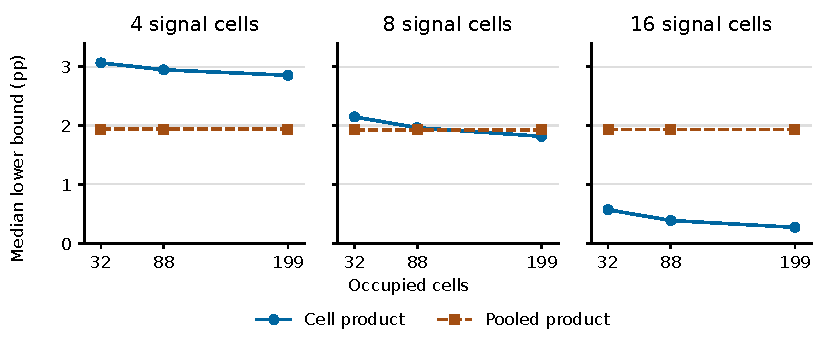
\includegraphics[width=\linewidth]{figures/cell-count-sweep.pdf}
\caption{Median product lower bounds across 10,000 replicates with 80 blocks and a true gain of 4 percentage points. Within each panel, splitting zero-gain cells changes the cell-level error allocation and preserves the pooled scores on every replicate.}
\label{fig:cell-count-sweep}
\end{figure}

With eight signal cells at 80 blocks, the cell product bound exceeds the pooled product bound in 75.47\%, 54.17\%, and 35.19\% of replicates as the occupied count rises from 32 to 88 and 199. The median ordering reverses (Fig.~\ref{fig:cell-count-sweep}). With four signal cells, the cell median remains larger at all three counts. With 20 blocks and eight signal cells, the fraction of positive cell product bounds falls from 54.09\% to 1.01\% between 32 and 199 occupied cells. These comparisons isolate the effect of the error allocation in this simulation.

\subsection{Sensitivity to the fitted rule and class prior}
\label{sec:xs-sensitivity}

We use the registered XS 16- and 44-class cohorts, the original fitting period, and both evaluation windows. We compare the frequency rule with a multinomial logistic rule using additive categorical terms for the same coarse symbol and timing bin. The logistic rule is fitted to equal-class weighted counts from the original pilot, with an L2 penalty of 0.001 in the normalized objective. An unseen coarse symbol uses the frequency-rule fallback. We also use class weights proportional to the square roots of the fitting counts, which reduces the target mass of the 44-class service with 190 original holdout flows from 2.27\% to 0.68\%. For 44 classes we cross both frequency fitting priors with both evaluation priors. Each comparison uses the same retained flows and blocks within a cohort and window. The tail probability is 0.05 per fixed bound in both windows.

\begin{table}[t]
\centering
\small
\setlength{\tabcolsep}{4pt}
\caption{Daily product lower bounds (pp) for XS sensitivity checks at tail probability 0.05 per fixed bound. The frequency and refitted rules use equal and square-root fitting priors, respectively. The prior shown in each row is the evaluation prior.}
\label{tab:xs-sensitivity}
\begin{tabular}{rlrrrr}
\toprule
 & & \multicolumn{2}{c}{Original} & \multicolumn{2}{c}{Disjoint} \\
Classes & Rule, evaluation prior & Cell & Pooled & Cell & Pooled \\
\midrule
16 & Frequency, equal & 1.48313 & 0 & 2.39217 & 0.35759 \\
   & Logistic, equal & 1.07323 & 0 & 1.90730 & 0 \\
   & Frequency, square root & 1.67405 & 0 & 2.44219 & 0 \\
   & Refitted, square root & 1.90142 & 0 & 2.53049 & 0.93079 \\
\addlinespace
44 & Frequency, equal & 2.01152 & 2.03485 & 1.35803 & 2.06194 \\
   & Logistic, equal & 0.93386 & 0.67926 & 0.88874 & 0.67020 \\
   & Frequency, square root & 0 & 0 & 0 & 0 \\
   & Refitted, equal & 0.24724 & 0 & 0.63444 & 0 \\
   & Refitted, square root & 1.38964 & 0.30499 & 1.83706 & 1.21411 \\
\bottomrule
\end{tabular}
\end{table}

The logistic rule gives positive daily bounds under equal priors in both cohorts and windows. For 44 classes, the cell product bound is larger than the pooled product bound on daily blocks with the logistic rule. At four days, the 16-class original-window logistic bounds are all zero. The 44-class pooled logistic bounds remain positive in both windows at that width.

With square-root evaluation priors, all four 44-class bounds from the equal-prior frequency rule are zero at all three widths. Its observed gains over the reweighted coarse optimum are $-4.523$ pp in the original window and $-1.923$ pp in the disjoint window. Refitting with the square-root prior raises these gains to 2.968 and 4.415 pp for the same Bayes gain target. The cell product lower bounds reach 1.390 and 1.837 pp on daily blocks, and 0.606 and 0.755 pp on four-day blocks. At the equal evaluation prior, this refit reduces the daily cell product bounds from 2.012 and 1.358 pp to 0.247 and 0.634 pp, and both daily pooled product bounds become zero. Thus the effect of refitting depends on the evaluation prior.

\subsection{Known-null checks}

We simulated 36 equally weighted coarse cells and 10 independent blocks per family. A binary outcome in each cell and block either makes the added feature agree with all labels or flips all labels, inducing perfect dependence among the affected records. Class balance and a weighted mean agreement probability of one half give zero Bayes gain. Across 100,000 families per scenario, the observed family false-positive rates were 3.541\% with independent fair outcomes across cells, 0.117\% with the outcome shared across cells within a block, and 0.024\% with independent cells and alternating block agreement probabilities of 0.1 and 0.9. Exact family probabilities are 3.456\%, 0.098\%, and 0.021\%, respectively. These checks exercise the known-null implementation under the assumed block model.

\section{Limits of certification}

\subsection{Independent-unit sample complexity in a binary model}

Consider balanced binary classes with a constant coarse feature. In unit $b$, a shared $U_b\sim\mathrm{Bernoulli}(p)$ either makes the fine feature agree with all labels or flips all labels. The units are independent. Repeating records inside a unit supplies one random bit about $p$. The Bayes gain is $|p-1/2|$. For the simple null $p=1/2$ and the fixed alternative $p=1/2+\delta$, every test of size at most $\alpha$ and power at least $1-\beta$ needs a number of units $n$ satisfying
\begin{equation}
 n\,d(1/2+\delta\,\Vert\,1/2)\ge d(1-\beta\,\Vert\,\alpha),
\end{equation}
where $d$ is Bernoulli relative entropy. This follows by applying data processing to the rejection indicator under the two joint laws \cite{kaufmann2016complexity}. The likelihood ratio increases with the number of agreements, so an exact upper-tail binomial test with boundary randomization attains the optimal size--power tradeoff \cite{neyman1933tests}.

Table~\ref{tab:power} contrasts the necessary KL count, the optimal randomized test, and two Hoeffding choices. The known range of the normalized unit score is $1/n$. The generic paired-score range is $2/n$. All counts refer to this model, the stated direction, and a fixed sample size.

\begin{table}[t]
\centering
\small
\setlength{\tabcolsep}{4pt}
\caption{Independent units for 80\% power at one-sided size 0.025 in the shared-bit model. The KL column is a necessary lower bound. The other columns give the first unit count attaining the target power.}
\label{tab:power}
\begin{tabular}{rrrrrr}
\toprule
Gain (pp) & KL & Optimal & Exact binomial & Known range H. & Generic H. \\
\midrule
1.00 & 12,279 & 19,621 & 19,648 & 31,577 & 98,344 \\
2.00 & 3,069 & 4,904 & 4,927 & 7,865 & 24,572 \\
4.76 & 542 & 865 & 869 & 1,377 & 4,330 \\
5.27 & 441 & 705 & 716 & 1,121 & 3,527 \\
\bottomrule
\end{tabular}
\end{table}

\subsection{A conditional converse for the frozen rule}

The frozen-rule gain and the Bayes gain are distinct targets. Write $D=\sum_c D_c$, $A=\sum_c A_c$, and let $x_b$ be the observed mutable correct weight in each block for the frozen rule. For the following construction, condition on the same cohort geometry as in Section~\ref{sec:target}. Independently for each block, replay the observed timing vector with probability $s_b$. Otherwise assign each mutable record a timing value that makes the frozen rule wrong. Such a value exists by definition. The expected frozen-rule accuracy under this law is $D+\sum_b s_bx_b$.

If $0<A-D<\sum_b x_b$, choose the probabilities to give zero frozen-rule gain and maximize the probability of replaying the complete observation. For $x_b>0$, maximizing $\sum_b\log s_b$ subject to $\sum_b s_bx_b=A-D$ and $s_b\le1$ gives $s_b=\min(1,c/x_b)$, where $\sum_b\min(c,x_b)=A-D$. A block with $x_b=0$ can be replayed with probability one. If $\prod_b s_b>\alpha$, a deterministic procedure with uniform conditional coverage at level $1-\alpha$ must return a nonpositive lower bound for the frozen-rule gain on the observed timing vectors. A positive value would cause failure whenever that observation is replayed under the constructed zero-gain law.

For the QUIC22 cohort, the replay probabilities for 1, 6, 24, and 48 hour groups are 8.53\%, 11.02\%, 11.02\%, and 32.91\%, respectively. All exceed 5\%. The law sets the expected accuracy of the particular frozen rule to the coarse optimum. The fine Bayes rule can choose different decisions under that law, so the construction permits a positive Bayes gain. This distinction is consistent with the positive daily Bayes-gain certificate in Table~\ref{tab:bounds}.

\section{Discussion}

The 16-class frequency-rule result locates a certified gain in one well-supported coarse symbol. The 44-class daily cell and pooled bounds remain positive in both windows after omitting the largest contributor. The simulation shows that both gain concentration and the number of occupied cells can change the relative performance of the product bounds. Matching the fitting prior to the evaluation prior can recover positive lower bounds for the same target and records. The fitted rule affects the evidence available to the certificate. The evaluation weights also determine the Bayes gain target.

The certificate targets the class-weighted gain on the fixed evaluation cohort. Extending the claim to future traffic would require assumptions connecting that cohort to the deployment population. The one-hour guard keeps each retained flow within one date. Shared traffic conditions can still induce dependence across dates. The positive lag-one correlations and the zero bound at one disjoint-window alignment motivate reporting sensitivity to both block width and alignment. Conditional independence remains an assumption for each partition. The collection schedule and duration of known shared conditions can inform a primary partition before evaluation timing is examined. A coverage statement for a selected partition requires an error budget for the selection and a valid sampling model for the candidate bounds used in that guarantee.

An alternative under independent blocks is to use empirical Bernstein bounds for the mean of bounded independent observations \cite{maurer2009bernstein}. Applying such a bound to the sum of heterogeneous block scores requires an appropriate common range or a bound that uses the individual ranges. Betting methods also give variance-adaptive bounds for settings with a specified conditional-mean structure \cite{waudby2024betting}. Residual dependence across blocks poses a separate problem. Heteroskedasticity and autocorrelation consistent covariance estimation \cite{newey1987hac} provides an asymptotic variance estimate under its own assumptions. The daily score ratios in our diagnostic can have different means and weights across dates. The finite-sample product bound requires factoring the expectation of the product across blocks, a condition that the lag correlations leave unresolved.

Both corpora were collected on the CESNET network in different periods and use different available label sets. QUIC22-S retains millions of flows and spans 20 evaluation days. Its coarser-width bounds are zero. The cross-corpus comparison changes the fitted rule, class mixture, and block score distribution along with the number of blocks.

\section{Conclusion}

Under conditional independence across blocks, nested fusion permits finite-sample lower bounds on class-weighted Bayes accuracy gains for a fixed evaluation cohort. In the 44-class XS cohort, the daily pooled product bounds for adding timing are 2.035 and 1.935 pp in two evaluation windows. Both remain positive after omitting the leading original cell and accounting for selection among omissions at the daily width. The simulations show how the distribution of gain and the number of occupied cells affect the choice between cell and pooled bounds. The XS sensitivity checks show how the fitted rule and the target class weights also affect the resulting bounds.

\section*{Data and code availability}

The corpora and release metadata are publicly documented \cite{luxemburk2023cesnet,cesnet2025cesnet}. The analysis archive provides input hashes, cohort definitions, fitted rules, per-cell results, simulation outputs, and the sample-size benchmark. The reproduction guide \path{TIMING_CELL_CERTIFICATE.md} lists the scripts, commands, and JSON outputs for the comparisons, temporal check, calendar alignment diagnostic, simulations, sensitivity analysis, and ablations.

\bibliographystyle{elsarticle-num}
\bibliography{references}
\end{document}
